\documentclass[a4paper,11pt]{memoir}

\ifpdf
\usepackage[utf8]{inputenc}
\usepackage[T1]{fontenc}
\fi

%\usepackage{german}
%\usepackage[english]{babel}
%\usepackage[german]{translator}
%\usepackage{hyperref}

\usepackage{import}
\usepackage{xifthen}
%\usepackage{pdfpages}
\usepackage{transparent}
\usepackage{subfig}
\usepackage{hhline}

\newcommand{\incfig}[1]{%
	\def\svgwidth{\columnwidth}
	\import{./bilder/}{#1.pdf_tex}
}

% This is the only file needed for actually using the smart-thesis style.
\input{style}

% Contains some packages which are commonly used in a thesis.
% Note that these are optional.
\usepackage{csquotes} % Context sensitive quotation facilities. Recommended by babel and should be loaded before babel.

\usepackage[english]{babel} % Sets the language used. Essential for proper hyphenation. Translates key words like 'figure' or 'table'. Note that 'english' is American English.

\usepackage{latexsym,amsmath,amssymb,amsthm,amscd} % Provides math enviroments, math symbols and more things useful for math.

\usepackage{mathtools} % Enhances amsmath and provides further mathematical tools.

\usepackage{graphicx} % Provides inclusion of graphics and a proper interface for '\in­clude­graph­ics'.
% Su­per­sedes 'epsfig' and 'graphics'.

\usepackage{enumitem} % Provides control over list environments. Supersedes 'enumerate', which gives enumerate environment an optional argument which determines the style in which the counter is printed.

%\let\newfloat\undefined % Hack to make floatrow work with memoir.
%\usepackage{floatrow} % Handles alignment of floats (figures), with centering as default.

\usepackage{xspace} % Ugly hack that sometimes helps with otherwise missing spaces.

\usepackage[backgroundcolor=white,linecolor=smartblue,bordercolor=smartblue,textsize=footnotesize]{todonotes} % Todo notes.

% Use sans-serif font in todos to clearly distinguish it from other text
\makeatletter
\renewcommand{\todo}[2][]{\@bsphack\@todo[#1]{\sffamily{#2}}\@esphack\ignorespaces}
\makeatother

\usepackage[style=alphabetic,backend=biber]{biblatex} % Bibliography.

%\usepackage{algorithm} % Algorithms.
% Use default Memoir floats for algorithms
\newcommand{\algorithmname}{Algorithm}
\newcommand{\listalgorithmname}{List of Algorithms}
\newlistof{listofalgorithms}{loa}{\listalgorithmname}
\newfloat[chapter]{algorithm}{loa}{\algorithmname}
\newfixedcaption{\falgcaption}{algorithm}
\newlistentry[chapter]{algorithm}{loa}{0}
\cftsetindents{algorithm}{0em}{2.3em}
\makeatletter
\g@addto@macro\insertchapterspace{\addtocontents{loa}{\protect\addvspace{10pt}}}
\makeatother

%\usepackage{algpseudocode} % Algorithms.

\usepackage{varioref} % Automatically locates references on other pages. Load before hyperref.

%\usepackage[hidelinks]{hyperref} % Clickable references.
\usepackage[pdfencoding=auto,pdfborderstyle={/S/U/W 1},linkbordercolor=ref,colorlinks,linkcolor=ref,citecolor=cite,urlcolor=url]{hyperref} % Clickable references.

\usepackage[all]{hypcap} % Anchors links to the beginning of their respective floats. Load after hyperref.

\usepackage[noabbrev,capitalize,nameinlink]{cleveref} % Names references automatically. Load after hyperref.

\usepackage[toc,acronym]{glossaries} % Glossary.

\usepackage{booktabs}
\usepackage{multirow}

\usepackage{pgfplots}
\pgfplotsset{compat=1.8}
\pgfplotscreateplotcyclelist{smart}{%
  tangoplum,semithick,every mark/.append style={fill=tangoplum!80!black},mark=*\\%
  tangogreen,semithick,every mark/.append style={fill=tangogreen!80!black},mark=square*\\%
  tangoorange,semithick,every mark/.append style={fill=tangoorange!80!black},mark=otimes*\\%
  tangoblue,semithick,mark=star\\%
  tangobutter,semithick,every mark/.append style={fill=tangobutter!80!black},mark=diamond*\\%
  tangored,semithick,every mark/.append style={solid,fill=tangored!80!black},mark=*\\%
}
\pgfplotsset{cycle list name=smart}

\usepackage{listings}

\definecolor{mygreen}{rgb}{0,0.6,0}
\definecolor{mygray}{rgb}{0.5,0.5,0.5}
\definecolor{mymauve}{rgb}{0.58,0,0.82}

\lstset{ %
  backgroundcolor=\color{white},   % choose the background color; you must add \usepackage{color} or \usepackage{xcolor}
  basicstyle=\footnotesize,        % the size of the fonts that are used for the code
  breakatwhitespace=false,         % sets if automatic breaks should only happen at whitespace
  breaklines=true,                 % sets automatic line breaking
  captionpos=b,                    % sets the caption-position to bottom
  commentstyle=\color{mygreen},    % comment style
  deletekeywords={...},            % if you want to delete keywords from the given language
  escapeinside={\%*}{*)},          % if you want to add LaTeX within your code
  extendedchars=true,              % lets you use non-ASCII characters; for 8-bits encodings only, does not work with UTF-8
  frame=single,	                   % adds a frame around the code
  keepspaces=true,                 % keeps spaces in text, useful for keeping indentation of code (possibly needs columns=flexible)
  keywordstyle=\color{blue},       % keyword style
  language=C++,                	% the language of the code
  otherkeywords={*,...},           % if you want to add more keywords to the set
  numbers=left,                    % where to put the line-numbers; possible values are (none, left, right)
  numbersep=5pt,                   % how far the line-numbers are from the code
  numberstyle=\tiny\color{mygray}, % the style that is used for the line-numbers
  rulecolor=\color{black},         % if not set, the frame-color may be changed on line-breaks within not-black text (e.g. comments (green here))
  showspaces=false,                % show spaces everywhere adding particular underscores; it overrides 'showstringspaces'
  showstringspaces=false,          % underline spaces within strings only
  showtabs=false,                  % show tabs within strings adding particular underscores
  stepnumber=1,                    % the step between two line-numbers. If it's 1, each line will be numbered
  stringstyle=\color{mymauve},     % string literal style
  tabsize=2,	                   % sets default tabsize to 2 spaces
  title=\lstname,                   % show the filename of files included with \lstinputlisting; also try caption instead of title
  literate=%
    {Ö}{{\"O}}1
    {Ä}{{\"A}}1
    {Ü}{{\"U}}1
    {ß}{{\ss}}1
    {ü}{{\"u}}1
    {ä}{{\"a}}1
    {ö}{{\"o}}1
    {~}{{\textasciitilde}}1
}

\renewcommand{\lstlistingname}{Quellcode}


% Contains some macros which are commonly used in a thesis.
% Note that these are optional.
\input{common-macros}

% These packages are only used in the demo and not necessarily
% required for smart-thesis.
\usepackage{todonotes}

% Loads bibliography for citations.
\addbibresource{thesis-bibliography.bib}


% Define all the metadata to be listed in \smarttitle and \smartcopyright
\thesistype{Master Thesis}
\discipline{Intelligent Systems}
\title{A configurable speech recognition pipeline for social robots}
\subtitle{Creating a Fusion Framework for analyzing speech data}
\author{Robert Feldhans}
\institution{Bielefeld University, Faculty of Technology, Central Lab Facilities}
\supervisors{Dr.-Ing.\@~Sven Wachsmuth,M.Sc.\@~Florian Lier,M.Sc.\@~Birte Richter}
\reviewers{Dr.-Ing.\@~Sven Wachsmuth,M.Sc.\@~Florian Lier}


\begin{document}

\frontmatter

\smarttitle

%!TEX root = thesis.tex

%=============================================================================


\chapter{Abstract}
- First introduction to speech recognition and related stuff

- then presentation of our pipeline, which is based on two pillars.

- Then evaluation based on two experiments to show the validity of this approach and performance of the proposed pipeline.

- Lastly we will discuss further work, improvements to the proposed pipeline, additional things to evaluate

%-----------


I will then continue to show the capabilities of the proposed solution in two experiments.


\newpage

\tableofcontents

\mainmatter
%!TEX root = thesis.tex

\chapter{Introduction \& Motivation}
\label{motiv:start}

Robotics in general depend heavily on \gls{hri}.%todo cite
\gls{hri} in turn is influenced and shaped by human-human interaction.
Since speech is one of (if not) the most important form of communication between humans, it is no surprise that is also one of the most important parts of \gls{hri}.
From a robots point of view, speech can be divided into speech synthesis and the main interest of this thesis: speech recognition.

Being able to perfectly understand the words a person spoke does not completely cover speech recognition.
See for example this video\footnote{\url{https://www.youtube.com/watch?v=iEMKZdwJPE8}} we provide or stills from it in figure \ref{pic:moti:imustgonow}.
In the video parts of a RoboCup@home Task of the RoboCup World Championship 2018 in Montreal can be seen.
In three different instances two referees are giving a robot commands, but they take turns in speaking to the robot.
The robot does not acknowledge this and does not seem to notice.
More so: When asking for the conformation of a specific command, it does not even seem to care that a different person gives this conformation, or that the original referee walked away and no longer seems to care.

\begin{figure}[]
	\centering
	\includegraphics[width=.82\textwidth]{bilder/motivation/intro_1_edit.png}\\\vspace{3pt}
	\includegraphics[width=.82\textwidth]{bilder/motivation/intro_2_edit.png}\\\vspace{3pt}
	\includegraphics[width=.82\textwidth]{bilder/motivation/intro_3_edit.png}\\\vspace{3pt}
	\includegraphics[width=.82\textwidth]{bilder/motivation/intro_4_edit.png}\\\vspace{3pt}
	
	\caption{Interaction between two referees and a robot in the RoboCup@home league.
		The referee in blue abandons the robot, which does not acknowledge this at all.}
	\label{pic:moti:imustgonow}
\end{figure}

Potential security risks aside, the shown interactions appear unnatural.
The robot does not seem to really perceive the human, instead it is quite clear that it just listens for a particular combination of words.
A similar phenomenon could very publicly be observed in the near past, when Amazons Alexa ordered a variety of objects online, after hearing commands from a  TV\footnote{\url{http://archive.is/zXuJu}}.

In social robots, this behavior is not acceptable, especially since the means to at least partially solve these problems already exist.
Voice recognition technologies which can differentiate voices to a degree most people could be identified are available (todo cite voice github project).
Additionally, computer vision can be used to search for speakers, either standalone, looking for moving lips (too cite), or in combination with sound source localization (see \ref{basics:ssl}).
We will later show (see chapter \ref{related:robocup}) these to not be in use by leading robotics teams.

Of course suitable robot behaviors need to be created, to take all this information into account.
When creating these behaviors, one must take into account how these information are fed into them.
The behavior in question must either be fed a pre-combined package or be able to combine the information, e.g. a spoken utterance and a distinct, detected voice.
If the behavior handles the combination both may not be fed into the behavior at the same time, resulting in the problem to combine them.
A number of factors have to be considered when combining these informations.
The ratios in which information may arrive may not be distributed evenly.
While just a single, long speech utterance may be received, a number of voices can be detected, or several results of the same voice.
Results thus have to be combined in a manner that takes this into account.
Additionally, results will almost always have different calculation times, based on what component created them and thus may be temporally unaligned.
This must be considered as well, creating the need to synchronize results based on their occurrence in time.

The problems just presented are clearly out of scope for robot behaviors an thus should be handled separately.
We thus declare the main goal of this thesis to be creating a framework to automatically generate these synchronized results of audio analysis solutions.

Furthermore, we can declare a number of secondary goals.
Naturally our approach to synchronize audio results shall not have a negative impact on these results.
This can be specified in two more concrete terms.
First and foremost, the accuracy of the results shall not decrease by being incorporated in our solution.
Second, synchronizing the results shall not take significantly longer to compute than not synchronizing them.
%todo elaborate

%---------------------------------- modularity secnd goal

Robotics is a field of intensive current research, and in the last years a number of leaps have been made.
These include, but are no limited to OpenPose (todo cite https://github.com/CMU-Perceptual-Computing-Lab/openpose), YOLO (todo cite https://pjreddie.com/darknet/yolo/) and DeepSpeech (todo cite https://github.com/mozilla/DeepSpeech).
Modularity and the ability to include such advances without the need to completely overhaul an existing system greatly decreases the time needed to incorporate such new technologies.
In turn, research speed can greatly benefit.
We can thus declare modularity a secondary goal, to increase the usability of the proposed framework.

%-----------------------------------

The remainder of this thesis is structured as follows:
We will first introduce a number of concepts and frameworks in chapter \ref{basics:start}.
After this we will present our solution to 
in chapter \ref{main:main}.
We will then proceed to evaluate our proposed solution in chapter \ref{eval} based on two experiments.
Lastly we will summarize our findings and point out possible future work in chapter \ref{conclusion}.

%--------------------------

%\section{old stuff}
%
%
%While other specialized fields of robotics or human robot interaction can get by just recognizing speech, social robots require more information.
%
%Humans are able to gather a plethora of information in in simple conversations which have next to nothing to do with what was actually said.
%Just by hearing a voice, one may determine a person’s emotional state, gender, or even where a person may be from, e.g. from an accent.
%A robot perceiving these information and addressing them if appropriately may lead a person interacting with the robot to feel better recognized as a person and such increase the persons acceptance of the robot.
%
%Several key features are relevant to take part in a conversation:
%The ability to match a voice/ spoken word to a (e.g. visually) perceived person, which in turn at least partially requires to recognize a voice and track the direction from where it is coming.
%Understanding whether or not a sentence or utterance was directed towards oneself.
%
%Meta information about the processes involved in speech recognition may prove useful in enabling the robot to give a user feedback on why something took longer than expected or otherwise improve interaction quality e.g. by shutting down non-essential nodes or downsampling audio data for transmission in situations where the robot is severely handicapped by low computational power or a high latency/ low throughput network respectively.
%
%What is generally known as Speech Recognition is actually comprised of several smaller subtasks, i.e. recording the raw sound, voice activity detection, and the actual speech recognition, as well as related tasks, such as sound source localization, sound filtering, beamforming, speaker recognition and addresser detection or emotion detection. %eher abstract?
%
%Speech recognition solutions tend to incorporate their basic subtasks into a single process.\todo{modularisierung eingener abschnitt?}
%This tends to entangle these subtasks to a point where code re-usability is infeasible and switching out individual subtasks is a time consuming and complex matter.
%
%\section{Synchronization of speech recognition results with related information}
%
%Speech recognition and related tasks (e.g. SSL) may take a while, especially on weaker hardware. 
%This poses a problem for systems relying on more than one of those types of data. 
%
%- synchronization between recognized speech and other information gathered by sound analysis may be tricky
%
%- to resolve synchronization issues down the line (NLP/ NLU), recognized speech should already be annotated with SSL results etc.
%
%Establishing a stable and comprehensive interface outside and inside the pipeline makes development of new components easy. 
%Evaluation of new components and benchmarking of and with existing ones can thus be greatly accelerated and encouraged.% eher auswertung?!
%
%\section{Latency}
%\todo{latency vs continuous audio signal eher in den hauptteil?}
%Latency is one of the top concerns in audio frameworks such as GStreamer and JACK (JACK Audio Connection Kit), but arguably rather unimportant in dedicated speech recognition tasks. 
%	
%Speech recognition tasks typically are bound by computationally intensive calculations, which will inherently produce a measurable latency/ delay between audio recording and recognized speech.  
%	
%For example, to recognize speech on a dynamically beamformed signal which is a typical use case with microphone arrays present on modern robots, one has to calculate sound source localization first, after which the beamformed signal can be calculated.
%If a voice activation detection is employed, it then needs to determines when a voice was picked up and and when the phrase ends, which typically takes a significant fraction of a second, thus adding to the latency. 
%	
%Because of the calculations and inherent delays, the latency introduced by the framework will almost always be rather insignificant and probably not be noticeable. 
%This holds especially true, if the point in time at which the result of the speech recognition is known can only be observed indirectly, e.g. the reaction of a robot to a spoken sentence given by a human will always be slightly delayed, just as a human typically needs a short time to react to new information, given to it verbally or otherwise.
%
%\section{Continuous Audio Signals}
%On the other hand, the possibility to lose audio frames introduces a significant problem to automated speech recognition.
%Lost audio frames result in artifacts found at the edges of neighboring frames. 
%These artifacts in turn result in unusual frequencies, which will cause problems in every step of a speech recognition pipeline which is not prepared for these to show up. 
%
%Frequency based voice activation detections and speech recognizers may not be trained with such corrupted data and produce undefined results.
%Sound source localization or beamforming solutions are particularly susceptible as they rely on several channels of audio, and if even one of them is missing, the others recorded at the same time may be unusable.
%Techniques to cope with potentially ensuing synchronization issues may also be needed to avoid undefined results.
%	
%Thus one might come to the conclusion that having a complete, discontinuity-free speech signal is more important than having a low latency.\todo{diese erkenntnis ist allerdings relativ wichtig für die motivation}
%
%
%\section{Target Audience/ Fields of Application}
%
%This work is predominantly targeted at researchers who develop new components related to speech recognition (e.g. SSL, VAD, beamforming, filtering). 
%Re-implementation of software slows down research so a framework, which allows them to easily incorporate a new algorithm/ technique into a existing pipeline of state of the art components for testing and benchmarking purposes, should improve the research speed and quality.
%
%Additional beneficiaries of this pipeline are developers who want to make use of speech recognition but do not have the resources to create their own pipeline.
%A typical user of this kind would come from the fields of robotics, which tends to be a rather interdisciplinary field, integrating more specialized fields into theirs, like speech recognition, AI, or human machine interaction.
%Giving them the opportunity to prototype and evaluate individual components and their interaction together in a standardized way.
%!TEX root = thesis.tex
%=============================================================================


\chapter{Introduction}

\section{Begriffserklärungen}

\subsection{Latency}

\subsection{\gls{ssl}}

\subsection{Beamforming}




%!TEX root = thesis.tex

\chapter{Related Work}

In this chapter a number of frameworks and libraries for audio transmission and their merit for speech recognition will be discussed.

\section{ALSA/ PulseAudio}
The Advanced Linux Sound Architecture (ALSA) 

\begin{itemize}
	\item 
\end{itemize}

%-------------------------------------------------------------------------------------
\section{JACK Audio}

The Jack audio connection kit (JACK) is a protocol for audio transmission between components with the explicit requirement for a low latency, to enable real time capture, playback and editing of sound. 
It provides an API to transmit audio between programs. 

Several implementations of JACK servers exist, notably JACK1 and JACK2. 
Differences between implementations are quite small and boil down to a handful of optional features and support for some operating systems which will most likely not matter for most users. % see https://github.com/jackaudio/jackaudio.github.com/wiki/Q_difference_jack1_jack2
Since all implementations provide the same interfaces, components are indifferent to the implementation of the JACK server used. 

JACK requires components to use a specific sample rate, sample size and audio format, which can however be adjusted before starting the JACK server. 
As such, any component which requires a different audio format has to handle resampling and converting on its own. 

JACK does not allow for additional information to transmitted with the raw audio it transports, so any additionally information must be transmitted and synchronized separately with another middleware. 

JACK is able to transmit audio over network, but generally requires all participating computers to run an instance of the same server implementation. 
An additional piece of software is needed to then create the connection between the different server instances. 
This complexity results in a moderate amount of setup and maintenance time required to handle an ever changing setup of computers and components a robot, especially in a research context, requires.

JACK requires all components which use its API to process audio in a specific and rather short time. 
Audio is written to and read from JACK via buffers, which will be in turn read and written by JACK in specific intervals.
If a component is not able to read or produce audio fast enough, JACK will overwrite or read old audio respectively, so audio is lost. 
This is important for applications which result in humans hearing the transmitted audio directly, to reduce latency and negate long or at least noticeable periods of silence.

\subsection{Problems regarding distributed Speech recognition applications}
For speech recognition purposes however, this audio frame dropping produces a series of problems. 
For once, transitions between audio frames become non-steady, which results in artifacts when frequency analysis or other feature extraction is employed.
Feature extraction algorithms using deep learning for example may not have been trained with audio which misses frames, and produce incomprehensible or unexpected results.


%-------------------------------------------------------------------------------------
\section{Gstreamer}

\begin{itemize}
	\item 
\end{itemize}

%-------------------------------------------------------------------------------------

\section{Interoperability between presented Frameworks}
\begin{itemize}
	\item most if not all of these frameworks can be used alongside each other and often have interfaces to each other
	\item 
\end{itemize}



%!TEX root = thesis.tex
%=============================================================================
\chapter{Configurable Speech Pipeline}
\label{main:main}
In this chapter I will describe my solution to the problems presented in chapter \ref{motiv:start}.
I will first give a broad overview how and where certain tasks are handled, before describing the two major components of the pipeline, the orchestrator and library, in more detail.
%After we discussed the problems tackled by the Orchestrator and the library in more detail and thus gained deeper insight into the workings of both, we will again revert to a higher level and describe their interaction with each other.
Lastly I will present a number of components developed for my solution as a proof of concept and to introduce them, as most of them are later used in the evaluation of this thesis (see chapter \ref{eval}).

The main goal of this thesis is to provide synchronized results of audio analysis components, such as \gls{asr} and \gls{ssl} results.
To effectively provide these fused results, these results are first needed in a standardized separated form.
Additionally, to be able to synchronize separated results based on time, they need to be annotated with a timestamp.
However, this timestamp needs to fulfill a number of requirements:
as the first and most central requirement, the timestamp must not correspond to the time a given result was made available, but rather to the time when the corresponding audio signal was recorded.
This is fundamental, as each result providing component can not be expected to take the exact same time as any other.
Additionally, as the audio this timestamp corresponds to is not a singular event, but a continuous stream, it must contain a start- \& an end-time to fully and accurately describe it.
This is especially true since results may be generated on audio of vastly different length.
Consider for example a simple "yes" or "no" in contrast to a longer question, such as "Hey robot, where can I find the orange juice?".
This directly leads to another problem:
as each results now requires an annotation in form of a timestamp, each component subsequently requires this annotated audio data.

This, in turn, leads to a number of cases with a high complexity in dependencies.
Consider a setup of a \gls{ssl} component, a beamformer and an \gls{asr} component.
In this setup, the \gls{ssl} component would have to acquire audio data and annotate it with timestamps as discussed above and then provide its results.
An independent beamformer would in turn also have to acquire audio and annotate it, and then match the \gls{ssl} results provided by the respective component to its audio data.
Then it could calculate the beamformed audio signal, which would also required to be annotated with timestamps.
Lastly, the \gls{asr} component would have to collect these timestamped audio signals, produce \gls{asr} results and then annotate them with timestamps.
An additional dependency implicitly declared in this example is that the \gls{asr} component must be able to process the audio annotated with timestamps the beamformer produces.
%Most commonly used libraries for audio transmission, as we have shown in chapter \ref{related:frameworks}, do not support adding of meta-information such as timestamps, so either these components would need to be merged or must prepare a interface for communication.

Most of these requirements could, in theory, be handled by the components themselves.
However, I decided to outsource most of the work done by the components into a library, to allow them to focus on their respective goals.
This provides a number of advantages:

First, by outsourcing this work standards must inherently be defined.
As they can easily be heeded by the components, they provide benefits for the individual components and for the final synchronization of the results.
More so, by defining these standards and providing a library to heed them, the fragmentation of speech recognition components is encouraged. 
Take for example the \gls{psa} described in chapter \ref{related_work:psa}.
Not only does it contain an \gls{asr} component, but also a \gls{vad} component.
This makes sense from a developmental perspective, but impedes further development and replacing of its parts.
Even when done correctly and iteratively, after a few exchanges new technologies may need different interfaces.
By encouraging this melding of components to not occur, the resulting framework becomes highly modular and enables fast prototyping.
It also makes benchmarking individual components of such a pipeline easier, as I will later show with a number of experiments for evaluation (see chapter \ref{eval:dataset}).

Furthermore, by providing a way to easily send properly timestamped audio between components, a massive amount of work is lifted off the individual components, which in turn ensures the correct transmission of audio timestamps.
Additionally, more technical benefits include the prevention of code duplication and the reduction of bugs, which provide more time for actual research.

By embedding each component into the framework provided by the library, the proposed solution for finally synchronizing the results is also provided with standardized interfaces.
I named this solution the Orchestrator, as it not only synchronizes the results, but also keeps track of all components within the proposed pipeline.

Both library and Orchestrator work in tandem and need to communicate with each other on several occasions.
\gls{ros} was chosen as an underlying middleware, see chapter \ref{intro:ros}.
There are several reasons for this.
First, due to \gls{ros} relying on TCP, all communication can be expected to arrive, none will be lost.
Additionally, pre-existing infrastructure, such as a behavior controller used in one of the evaluations experiments already depends on \gls{ros}.
As such choosing \gls{ros} will prove beneficial for future work.

I will now continue to discuss the Orchestrator and the proposed pipelines library in more detail in designated sections.


%!TEX root = thesis.tex

%=============================================================================


\chapter{Library}

- default nodes for convenience and 
\newpage
%!TEX root = thesis.tex

%=============================================================================


\chapter{Orchestrator}

\begin{itemize}
	\item manages all participating nodes
	\item determines used audio formats for transmission
	\item handles synchronization task
	\item handles meta data accumulation, introspection and acts on anomalies
\end{itemize}

meta information gathering:

\begin{itemize}
	\item how the orchestrator gathers meta information and what exactly he gathers
	\item how this information is then used
\end{itemize}

algorithms implemented for the orchestrator

\begin{itemize}
	\item minimizing amount of resampling
	\item how is synchronization/ fusion solved?
	\item feedback to user if a non-optimal configuration is found (algorithm on how to find those)
\end{itemize}

\subsection{Meta Information Gathering}
It is desirable to gather meta information about results delivered by nodes. I.e. probability of a certain result and time to compute. TTC can be used to better predict if a node will deliver a result at all. See synchronisation of results in the orchestrator algorithms chapter.

Method 1: Every results need to be enhanced with meta informations

pro

- relatively easy to implement

con

-nodes need to explicitly keep track on this information and fill them (user unfriendly)

- results bigger than they need to be

- Method 2: TTC can be computed by orchestrator, other meta information included 

pro

-TTC can be expected to always exist and be correct (can not be expected if nodes are expected to calculate it)

-node implementation is not blown up

con

-not all nodes provide results, so beamformer and filter nodes need to provide the meta information explicitly

-how would this work?

-each result message has a timestamp, in combination with the audio flow graph calculated by the orchestrator, the time from one result to the next in line is roughly the time the next node took for computation

\newpage
%!TEX root = ../../thesis.tex

\section{Developed \& Incorporated Components}
\label{main:components:start}
In this section, components that were developed for the proposed pipeline will be discussed.
These components cover different aspects of speech recognition.

\marginnote{One good example would be a DeepSpeech component I developed\footnotemark. It makes use of a TensorFlow \cite{tensorflow} implementation of Baidus Deepspeech \cite{deepspeech}.}
\footnotetext{\url{https://github.com/Slothologist/DeepSpeech4Ros}}
Some initially planned and partially developed components were left out of this list, because it became clear they could not be included into this thesis in a meaningful way.
Thus development for these components was stopped or they were left out in favor of diverting time to more important parts of this thesis.


A handful of components are included in the library's repository, as they provide utility functions or are commonly used.
None of these components provide any information to the \textit{Orchestrator}, apart from registering.
These components are:
\begin{itemize}[leftmargin=1in]
	\item[\textit{Audio Grabber}] The \textit{Audio Grabber} is the most fundamental node, as it is the basis of most pipeline configurations.
	It is able to grab audio from a microphone via \gls{alsa} and feed it into the pipeline.

	\item[\textit{Audio Player}] This component is the \textit{Audio Grabbers} counterpart, as it receives audio data from the pipeline and outputs it via \gls{alsa} through a speaker.
	As such, it is mostly used for debugging purposes and to enable quick auditory microphone checks.

	\item[\textit{Channel Splitter}] As discussed in section \ref{main:lib:formats}, the proposed pipeline's library does not support mixing of channels.
	The \textit{Channel Splitter} is used to mitigate this absence by receiving a multichannel audio signal and produces a corresponding number of single channel outputs.
	One possible use case is to split a multichannel audio needed for \gls{ssl} into single channel audio usable for speech recognition, when no beamforming is desired.

	\item[\textit{Recorder}] The \textit{Recorder} is able to write audio it receives via the proposed pipeline to a file.
	Its foremost usage is to save audio it receives via the proposed pipeline to a file for later inspection or analysis.
	This can either be done for documentation purposes or, as was mostly done during development, to check if the pipeline transmitted and resampled audio correctly.
\end{itemize}
Additional components not included in the libraries repository cover the topics of:

\subsubsection{Wav Player}
\label{main:components:wav}
The \textit{Wav Player}\footnote{\url{https://github.com/Slothologist/esiaf_wav_player}} fulfills the same role as the \textit{Audio Grabber}, as it feeds audio into the pipeline.
However, it will read a given set of wav files in and output them into the pipeline.
It is capable of either producing silence in between each wav file or waiting for a time before playing the next file.
As such its predominant use case is to enable evaluations of other components with the help of data sets.

\subsubsection{Sound Source Localization}
\label{main:components:ssl}
I developed a component\footnote{\url{https://github.com/Slothologist/esiaf_doa}} which performs \gls{ssl}.
It uses the python library \texttt{pyroomacoustics} \cite{pyroomacoustics}, and specifically its SRP algorithm, though usage of all other \gls{ssl} algorithms provided by \texttt{pyroomacoustics} can be configured.
For each sound chunk the component receives via the proposed framework, it creates \gls{ssl} results and then sends them to the Orchestrator.

A slight variation of this node\footnote{\url{https://github.com/Slothologist/ma_baseline_doa}}  will be used in one of the experiments of the evaluation chapter (see \ref{eval:task_start}).
This variant will, instead of publishing results for each sound chunk it receives, store these results in a queue.
To communicate the results it provides a \gls{ros} service which allows any component to ask for results which occurred in a specified time frame.
Additionally, this variant will receive audio not from the proposed framework, but instead capture it from a microphone via \gls{alsa}.

\subsubsection{Voice Activity Detection}
\label{main:components:vad}
The \gls{vad} I developed\footnote{\url{https://github.com/Slothologist/AudioSegmenter}} is a reimplementation of a pre-existing algorithm present in the \gls{psa} (see chapter \ref{related_work:psa}).
Its segmentation is therefore virtually identical to the \gls{psa}'s.

If it detects the end of a segmentation, it will enhance the corresponding audio chunk with a \texttt{segmentation\_ended annotation}, as described in chapter \ref{main:lib:augmented_audio_msg}, before sending it.
Audio will not be transmitted to the next node(s) if it were not found to include speech.

\subsubsection{Automatic Speech Recognition}
\label{main:components:ps}
The \gls{asr} component I developed\footnote{\url{https://github.com/Slothologist/esiaf_pocketsphinx}} is a very simple wrapper around the python wrapper of \gls{ps}.
It will feed all audio it receives into \gls{ps}, which will then dynamically produce results.
These results are however only used if a \gls{vad} signals the end of a segment.
As such, this \gls{ps} component requires a \gls{vad} to work.
Whenever a result is produced, it is sent to the Orchestrator via published \gls{ros} message (see chapter \ref{main:lib:message_types}).

\subsubsection{Emotion Recognition}
\label{main:components:emotion}
The emotion recognition component I developed\footnote{\url{https://github.com/Slothologist/esiaf_speech_emotion_recognition}} makes use of \texttt{Speech Emotion Recognition} \cite{speech-em-rec}.
\texttt{Speech Emotion Recognition} uses a neural net to extract the emotional state of a person based on their speech.
As such, it is capable to categorize speech into three emotions: angry, happy, sad.
Additionally, speech can be categorized as neutral.
Small changes were required for it to meet all the proposed framework's expectations, so I improved it to include a probability for each result. %TODO
Each sound chunk this component acquires will be fed into \texttt{Speech Emotion Recognition} which will return an emotion and probability for each of these sound chunks.
These results are then sent to the Orchestrator for further synchronization.

\subsubsection{Gender Recognition}
\label{main:components:gender}
The gender recognition component\footnote{\url{https://github.com/Slothologist/esiaf_gender_rec}} I created is actually a somewhat new development.
It is based upon \texttt{Speech Emotion Recognition}, as it uses a nearly identical neural net and dataset.
However, I adjusted the output dimension of the neural net and reorganized its training data to classify either to male or to female, instead of the four emotions.
It also includes my changes, so its results include a probability.
I retrained the net and achieved a training accuracy of 99.63\% while maintaining a test accuracy on unseen data of 91.20\%.
Similar to the described emotion recognition component, it will produce a gender result for each sound chunk it receives along with a probability for it and send them to the Orchestrator.

It should be noted that the data set was quite small with only 339 audio samples, 188 of which by 5 female speakers , 151 from 5 male.
I suspect this being the cause for it to not achieve the level of accuracy on real world data that it achieved on the test data.
This observation is however anecdotally and was not evaluated formally.
However, I was satisfied with this solution, as it produces somewhat reasonable results.

This is especially true given the fact that it is not a part of this thesis to develop new approaches to recognition of gender, emotion or speech.
I chose this course of action with this specific component however, because an almost feasible component in the form of the described emotion recognizer was already in place and retraining of its neural net seemed to be a quick and easy way to produce a new component.
The alternative would have been to restructure and adjust a different approach, which may not have worked at all.








%!TEX root = ../thesis.tex
%=============================================================================


\chapter{Evaluation}

In this chapter, two tests will be presented which were used to evaluate the proposed speech recognition pipeline. 
Firstly, different configurations of the proposed speech recognition pipeline will be compared against each other and against a baseline in the form of an already existing solution.
This test will focus on performance and computational cost.
Secondly, a configuration of the proposed pipeline will be compared against an existing solution in a slightly altered RoboCup@Home Speech- \& Person Recognition task with focus on sound source localization results.


%!TEX root = thesis.tex
%=============================================================================


\section{Dataset Evaluation}
\label{eval:dataset}

In this section, an evaluation of the proposed pipeline and an existing solution on a dataset will be presented.
The goal of this evaluation is to take a closer look on the performance of the proposed pipeline with the explicit focus on computational cost as well as time needed for recognizing speech.

Based on the additional features the proposed pipeline introduces, most prominently synchronization of speech results and the modular nature of the pipeline, as presented in chapters TODO, we expect the proposed pipeline to consume more CPU power as well as taking longer to compute results in comparison to the existing solution.
To further examine the cost, we will in particular inspect the cost different additional components will add to the pipeline, to determine the scaling of the proposed pipeline.

We will lastly discuss if this additional cost makes using the pipeline unsuitable for real world applications or if the benefits overweight these costs.

\subsubsection{Dataset}
\label{eval:dataset:dataset}

The dataset used for this evaluation consists of 1723 samples with length between a half and fourteen seconds.
It incorporates 12 speakers (male and female) speaking 24 phrases. 
Individual samples were recorded using two microphones, one omni directional and one cardioid.
They were recorded in two rooms, some of them with noise, others without.

To more easily feed all samples into the existing solution, the wav files containing the samples were concatenated into one big wav file, with three seconds of silence added in between the individual samples, to easily distinguish the samples from one another.
This also simplifies matching the recorded speech recognition results with the actual utterances by .
The proposed pipeline was fed each sample individually, but three seconds of silence were similarly inserted into the audio.

The complete datasets playtime including the silence amounted to nearly two hours and fifty minutes.

\subsubsection{Setup}
\label{eval:dataset:setup}

Two slightly different setups were used for the various configurations of the proposed pipeline on the one hand and the existing solution on the other hand, due to differences in acquiring audio data.
What the have in common is that all pipeline were tested on the same computer, a Thinkpad Carbon X1 Gen with a Intel(R) Core(TM) i7-7500U, to ensure equality in CPU performance.

All were comprised of equivalent components. 
If not otherwise stated, all variations of the proposed pipeline used the exact same components with identical configurations (safe for some minor details, e.g. a modified path for the audio between the wav player, dummy node and VAD in the elongated version of the proposed pipeline, see figure \ref{pic:eval_p2_diag} and \ref{pic:eval_p4_diag}).

The existing pipeline's PocketSphinxAdapter internally incorporates a VAD, which was reimplemented and used as the VAD of the proposed pipelines.
It uses PocketSphinx for speech recognition, as does the speech recognizer used in the proposed pipeline. 
Both PocketSphinx instances use the same speech models, dictionary and grammar.

In both cases two small scripts were used to record the components CPU usage as well as speech recognition results and timings.
CPU usage was universally recorded using the python library psutil and its cpu\_times functionality.
However, psutils reliability can be called into question, as it seems not to take into account modern CPU's capability to increase or decrease their clock speed, depending on load.
As such, the recorded CPU costs should rather be taken as rough estimates and not as exact measurements.
We included this data points despite their supposed inaccuracy because apart from the last tested pipeline, all pipelines did not produce enough load on the CPU to cause it to increase its clock speed.
This is supported by fact that identical components across various pipelines produce very similar CPU loads, as seen in figure 
\ref{table:eval_dataset_detail}.
Incidentally a process producing the computational load of one CPU second over any timespan is equal to the process running on one core of a CPU under full load for one second.

Speech recognition results were recorded by a ROS node which collected ROS messages published by the proposed pipelines orchestrator respectively the PocketSphinxAdapter.

\subsubsection{Result Recording}

The times needed to calculate results were recorded in two different ways.
Due to the fact that the proposed pipeline annotates its results with the time the audio was recorded, it is rather simple to calculate the time needed for recognition.
One can just subtract the time when the analyzed audio signal ended from the time the synchronized result was received by the recording component an thus get the absolute time needed for recognition.
To be precise, this way we measure the time from when the segmentation ends to the point where the recording node received the recognized speech result.

The method of feeding audio into the proposed pipeline does not matter as long as the time stamps of the audio are correct, so instead of grabbing the audio via a microphone we used a wav-file player to feed the dataset directly into the pipeline.

The existing solution however was in need of a small workaround to work on audio files rather then audio directly grabbed by a real microphone.
A virtual microphone was needed to feed the dataset into the PocketSphinxAdapter.
This virtual microphone provided access to a wav file containing the dataset. 
As information about singular utterances inside the dataset could not be propagated through ALSA and the PocketSphinxAdapter, we recorded a time stamp with the start of feeding the wav file into the virtual microphone and thus in turn into the PocketSphinxAdapter.
Speech recognitions results were then recorded along time stamps acquired when these results were received in the dedicated ROS node.
Supplementary, the while concatenating the dataset into the singular wav file, we created annotations to keep track of when each sample ended and which phrase it contained.
To achieve comparable results, slight modifications to the internal segmenter fn the PocketSphinxAdapter were made, i.e. timestamps on each successful segmentation would be recorded.

By combining the information provided by these annotations, the time stamp created during the start of feeding the wav file, the timestamps recorded when recording the speech recognition results and after each successful segmentation, the absolute time needed by this solution could be computed.
This is mostly done by subtracting the timestamp collected after a successful segmentation from the corresponding recorded when the results were received.
Thus we record the time from the segmentations end to receiving the results, as previously with the proposed pipeline.

In any case, speech recognition results and timings were recorded as raw data and written to files.
Afterwards, these raw results could be processed and evaluated with the help of further scripts.


\begin{figure}[]
	\centering
	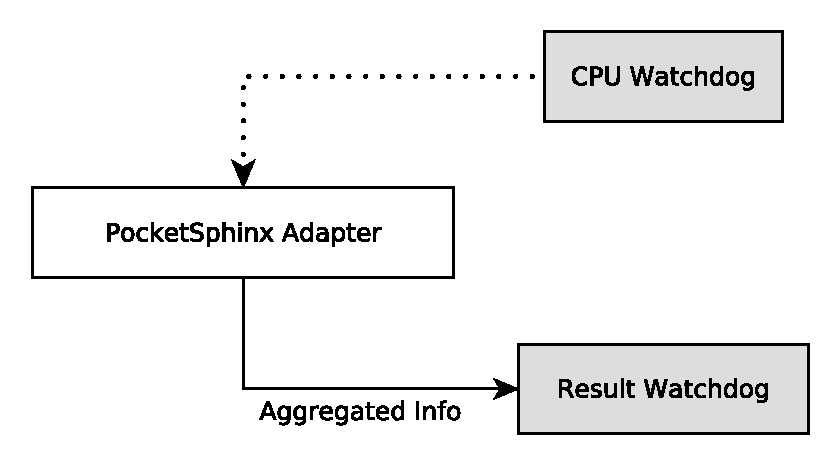
\includegraphics[width=0.66\textwidth]{diagrams/eval_pipeline_1.pdf}
	\caption{Test scenario for existing pipeline}
	\label{pic:eval_p1_diag}
\end{figure}

\begin{figure}[]	
	\centering
	\subfloat[Scenario for baseline of proposed pipeline]{
		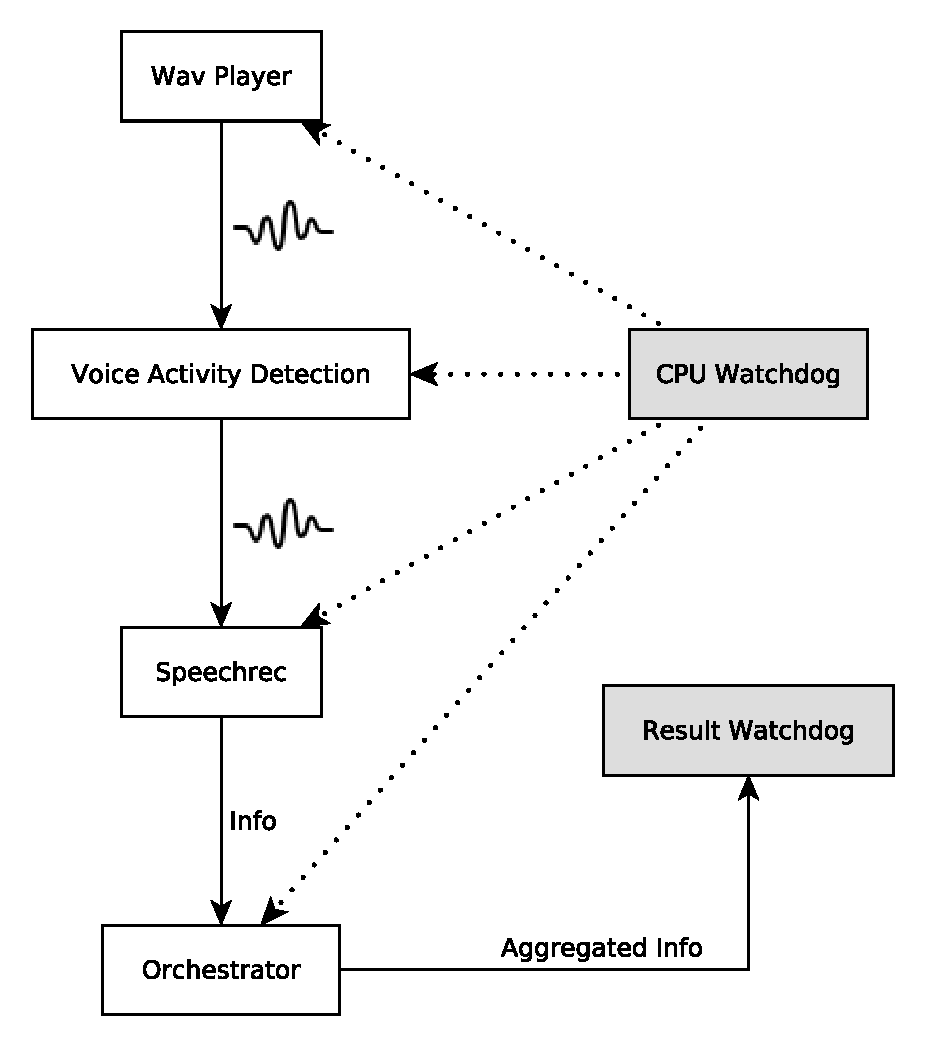
\includegraphics[width=0.5\textwidth]{diagrams/eval_pipeline_2.pdf}
		\label{pic:eval_p2_diag}
	}
	\subfloat[Scenario for elongated baseline of proposed pipeline]{
		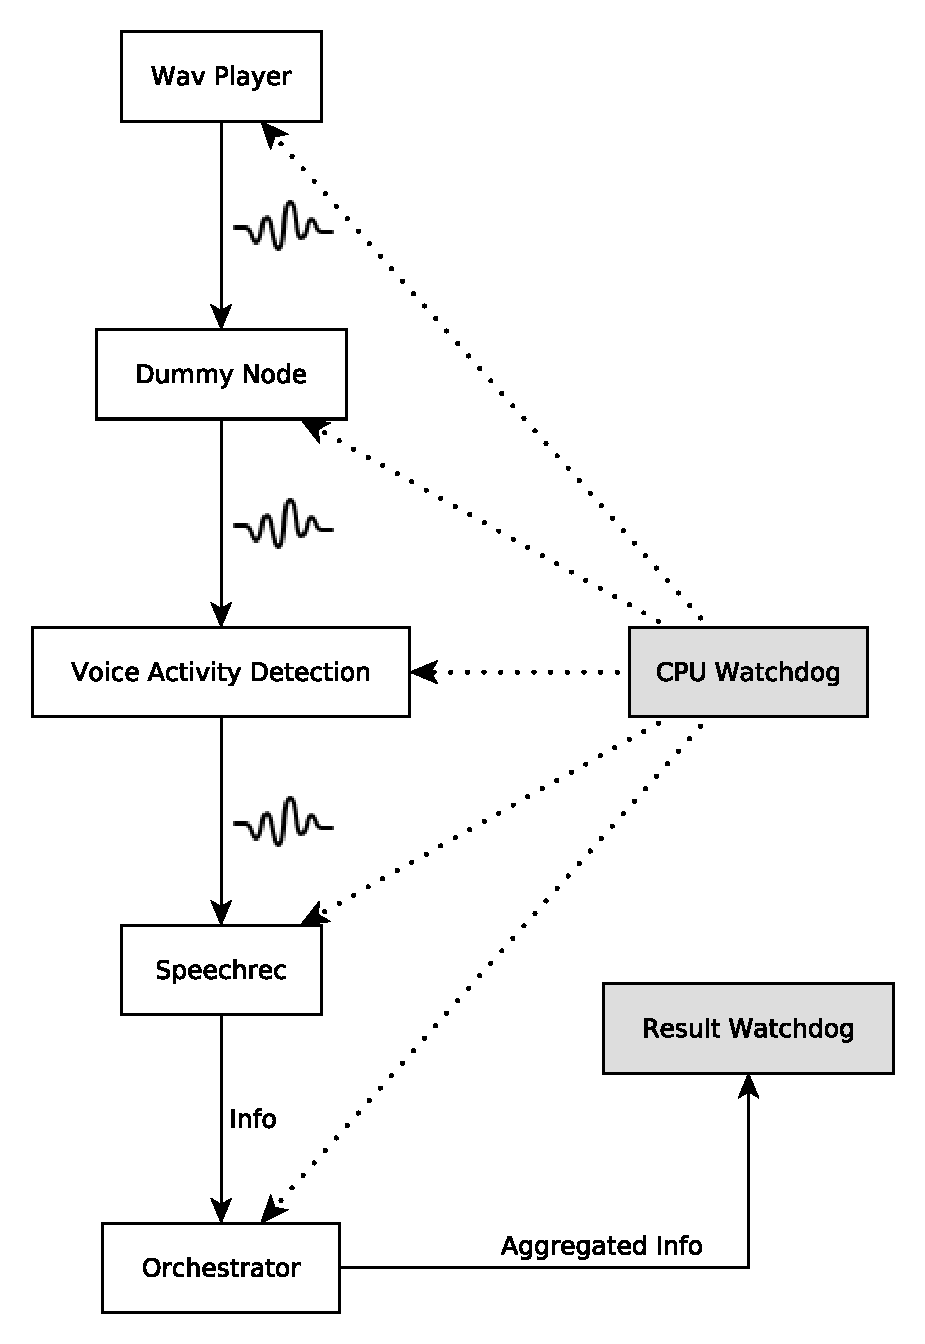
\includegraphics[width=0.5\textwidth]{diagrams/eval_pipeline_4.pdf}
		\label{pic:eval_p4_diag}
	}
	
	\caption{Test scenarios for proposed pipeline}
	\label{pic:eval_p2_4_diag}
\end{figure}


\begin{figure}[]	
	\centering
	\resizebox{\textwidth}{!}{
		\subfloat[Test scenario for widened baseline of proposed pipeline]{
			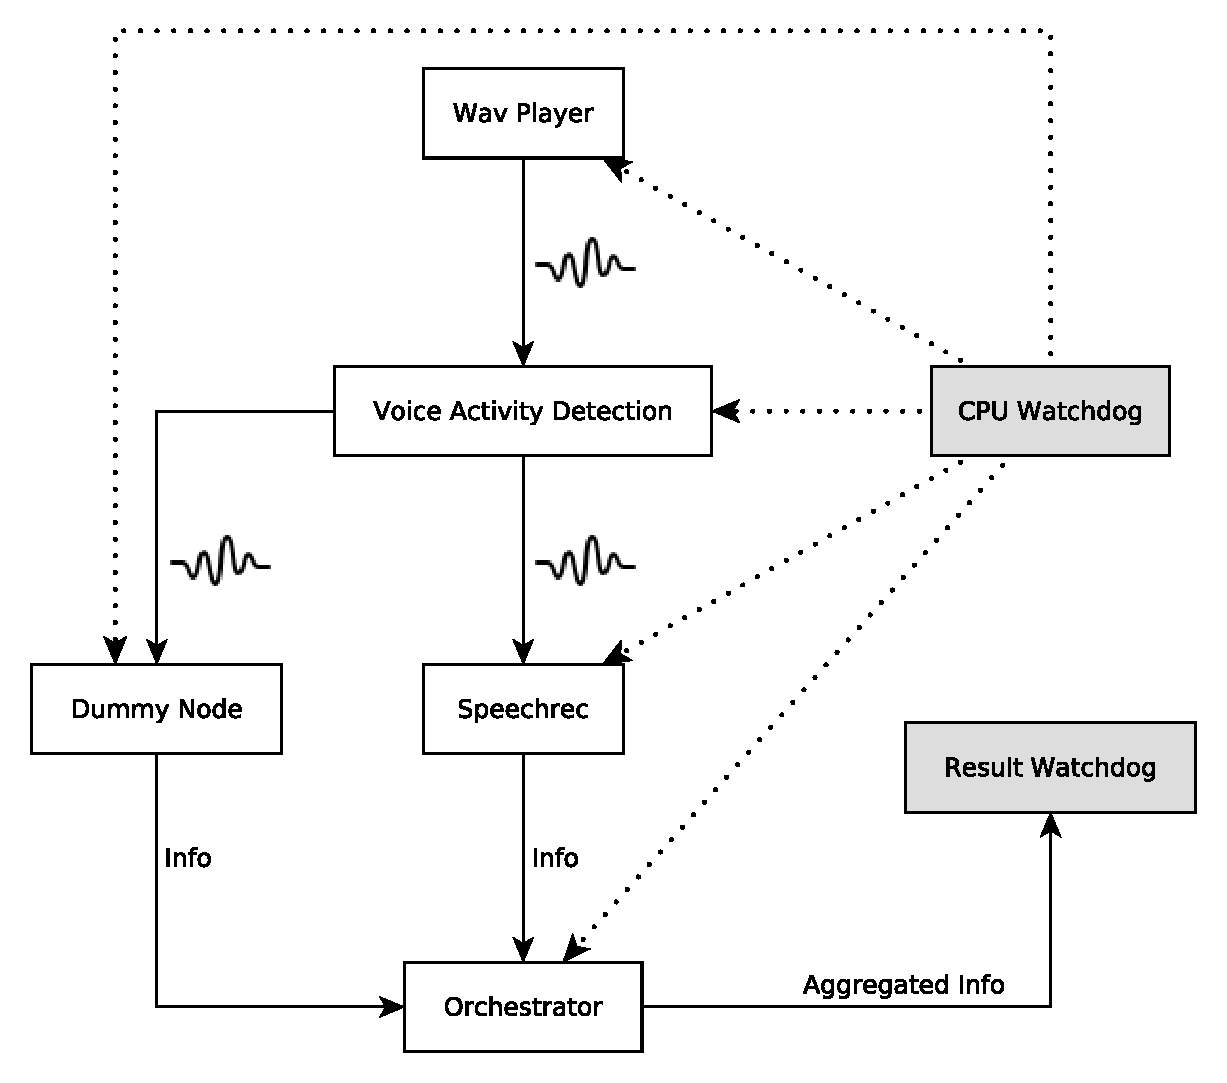
\includegraphics[height=0.4\textwidth]{diagrams/eval_pipeline_3.pdf}
			\label{pic:eval_p3_diag}
		}
		\quad
		\subfloat[Test scenario for elongated baseline of proposed pipeline]{
			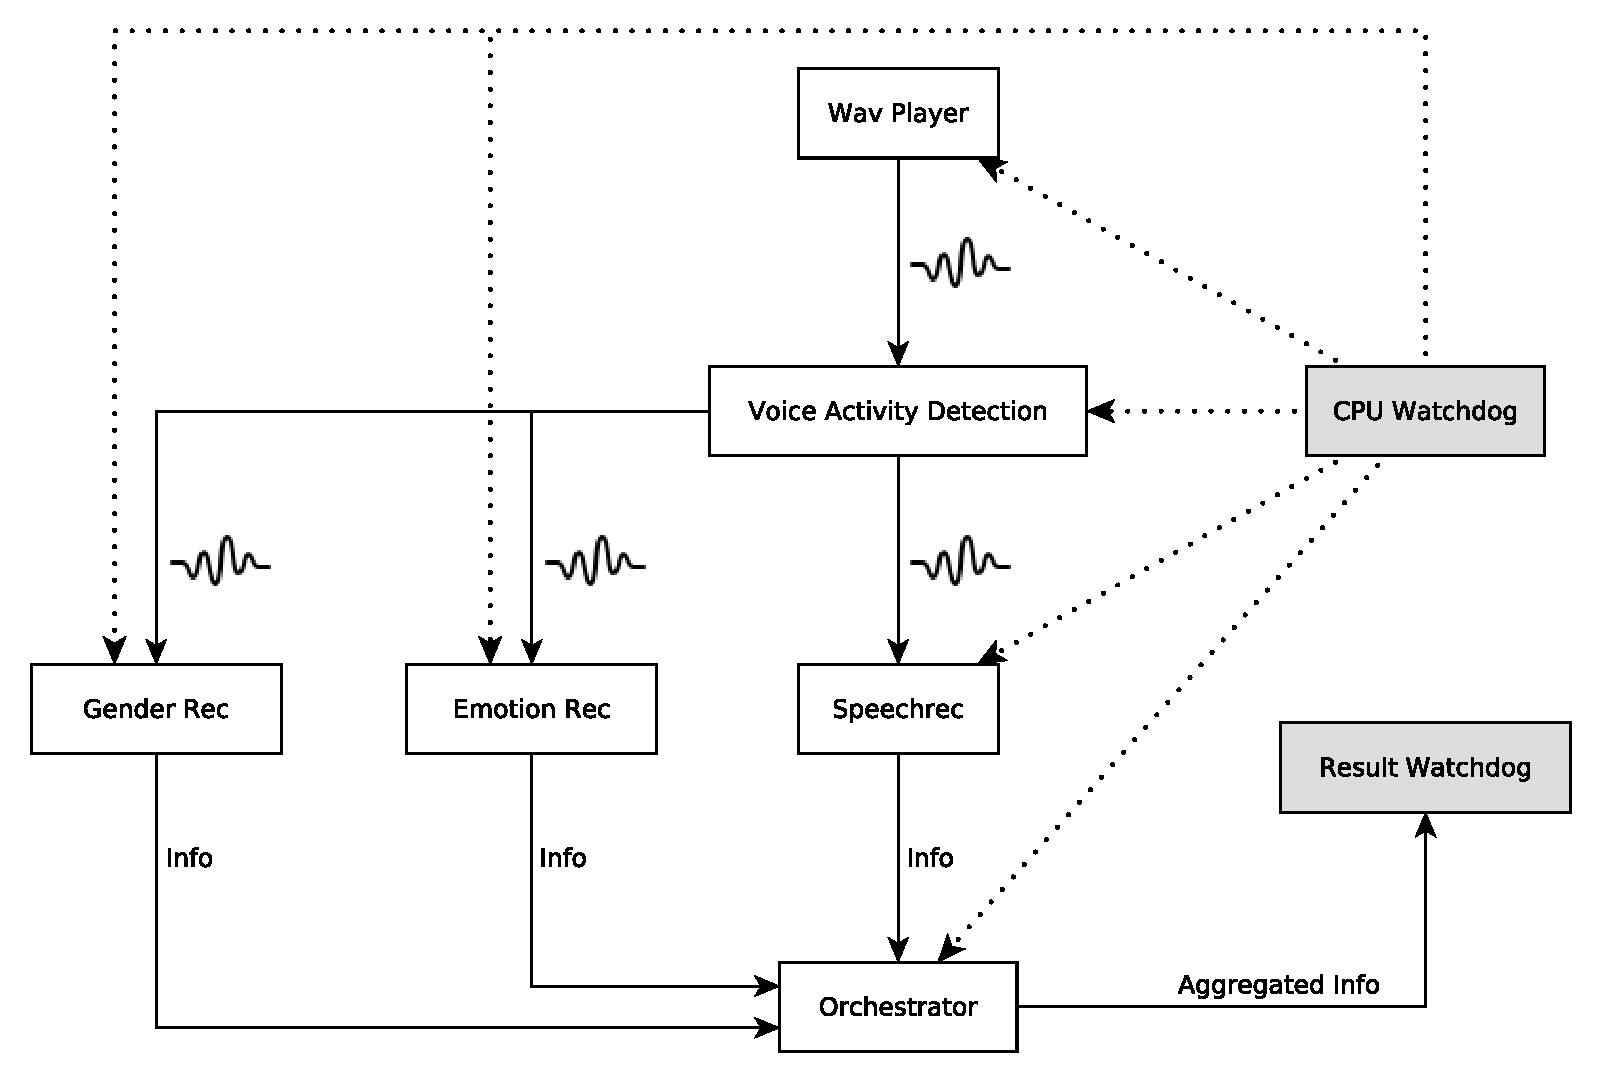
\includegraphics[height=0.4\textwidth]{diagrams/eval_pipeline_5.pdf}
			\label{pic:eval_p5_diag}
		}
	}
	
	\caption{Test scenarios for proposed pipeline}
	\label{pic:eval_p3_5_diag}
\end{figure}

\begin{figure}[]
	\begin{tabular}{ | l | p{0.2\textwidth} | p{0.2\textwidth} | r|}
		\hline
		Pipeline 	& Recognition percentage & Absolute time till result & Sum CPU time \\ \hline
		Existing 	& 77.02\% & 0.063 sec &   228.99 sec \\ \hline
		Proposed 	& 99.77\% & 1.014 sec &  1209.30 sec \\ \hline
		Elongated 	& 99.77\% & 1.039 sec &  1399.63 sec \\ \hline
		Widened 	& 99.65\% & 1.090 sec &  1665.66 sec \\ \hline
		Realistic 	& 99.48\% & 1.780 sec & 37517.13 sec \\ \hline
	\end{tabular}
	\caption{Results of the pipelines in comparison}
	\label{table:eval_dataset_results}
\end{figure}

\begin{figure}[]
	\begin{tabular}{ | l | r | r | r | r | r |}
		\hline
		Component 	& Existing 	& Proposed & Elongated & Widened & Realistic\\ \hline
		Speech Rec 	& 247.44 	& 546.65 & 545.73 & 574.82	 &   285.77 \\ \hline
		Orchestrator& - 		& 107.66 & 114.69 & 415.73	 &   962.56 \\ \hline
		Wav Player 	& -			& 380.11 & 378.71 & 405.40	 &   138.22 \\ \hline
		VAD		 	& - 		& 174.88 & 188.56 & 191.97	 &    51.26 \\ \hline
		Dummy	 	& - 		& -		 & 171.94 &  77.74	 &        - \\ \hline
		Gender Rec 	& - 		& -		 & -	  & -	 	 &  5959.50 \\ \hline
		Emotion Rec	& - 		& -		 & - 	  & -		 & 30119.82 \\ \hline
	\end{tabular}
	\caption{Detailed CPU cost}
	\label{table:eval_dataset_detail}
\end{figure}

\subsection{Tested pipelines}

\subsubsection{Existing Solution}

The existing solution consists only of the PocketSphinxAdapter (PSA), see figure \ref{pic:eval_p1_diag}.
The PSA grabs audio from a microphone using ALSA, filters the audio using an integrated voice activity detection and finally uses, as its name suggests, PocketSphinx to recognize speech.
Results are then published via ROS.

The PSA was and is used extensively for several years now in the RoboCup@Home setup of Team ToBi.
In this evaluation it is primarily used to provide a baseline for the proposed pipeline and context for the acquired results.

\subsubsection{Baseline for proposed Pipeline}
This configuration of the proposed pipeline is intended to reassemble the PSA as closely as possible.
As seen in figure \ref{pic:eval_p2_diag}, it consists of a voice activity detection, a speech recognizer (using PocketSphinx), the Orchestrator and a Wav file player to feed audio into the pipeline.
Recognition results are gathered by the Orchestrator and then communicated via ROS.

As can clearly be seen in figure \ref{table:eval_dataset_results}, each configuration takes over a second to compute speech recognition results.
We will discuss this -in comparison with the PSAs result- enormous time at a later in section \ref{eval:discussion}, after we procured more insight to the proposed pipelines scaling.
Consumed CPU time will also be discussed later, for similar reasons.

If one compares the recognition percentages of all the pipelines in figure \ref{table:eval_dataset_results}, the various configurations of the proposed pipeline all share virtually identical results, which however differs significantly from the PSAs result.
This is somewhat unexpected, as special care was taken to ensure both speech recognizers use not only PocketSphinx, but also equal configuration files, including speech model, dictionary and grammar.
As the audio segmentation for the proposed pipeline is a reimplementation of the one used internally in the PSA, and was furthermore basically bypassed in that the silence in between samples enabled the usage of very lenient VAD configurations.

The proposed pipelines PocketSphinx component is written in Python and uses its PocketSphinx wrapper, which in turn makes use of the same C++ libraries as the PSA, so it would be difficult to claim this as the determining difference responsible for this discrepancy.
Clearly more testing is needed to produce substantiated suppositions about the difference in recognition results.



\subsubsection{Elongated baseline of proposed Pipeline}
This configuration of the proposed pipeline is nearly identical to its baseline, but incorporates a dummy component to evaluate how much overhead in time and CPU cost an additional processing step produces.
As indicated in figure \ref{pic:eval_p4_diag} and by its name, the dummy node does neither alter nor compute information on the audio data it received, but instead just relays it from the WAV player to the VAD.

If one compares the results of the proposed and elongated pipeline in figure \ref{table:eval_dataset_results}, a slight increase in absolute time per recognition can be seen, as well as a moderate increase in CPU cost.
The increase in CPU cost is virtually completely due to the additional dummy component present in this pipeline, as can be extracted from figure \ref{table:eval_dataset_detail}. 

The slight increase of 15ms in absolute recognition time was, as discussed before, expected.
Considering a very elaborate configuration, where audio would be transmitted through audio grabbing, sound source localization, beamforming, audio enhancement, VAD and speech recognition, the latency introduced by using the proposed pipeline could be estimated to have an upper bound of 90ms.
This would barely be humanly noticeable and depending on the time taken by the components themselves probably be just a fraction of the absolute recognition time needed.
%Considering the VAD, which utilizes a computationally very inexpensive algorithm to segment the audio and should introduce only a slightly larger latency into the pipeline.


\subsubsection{Widened baseline of proposed Pipeline}
This configuration of the proposed pipeline is nearly identical to its baseline, but incorporates a dummy component to evaluate how much overhead in time and CPU cost an additional information provider produces.
As indicated in figure \ref{pic:eval_p3_diag} and by its name, the dummy node receives audio data from the VAD and works basically in parallel to the speech recognizer.
Upon receiving audio data, the dummy node provides hard coded ''information'' to the Orchestrator.
This way the Orchestrator does not have to wait on receiving the dummy nodes information during its synchronization steps, and can theoretically provide synchronized data as soon as speech recognition results are provided to it.

This is the first discussed configuration in which the Orchestrator has to actually synchronize data. 
In the baseline and elongated configuration it could take advantage of not having any other information provider and just relay all incoming data.
The additional computational power required by the Orchestrator can easily be observed in figure \ref{table:eval_dataset_detail}.
Though this configuration of the pipeline seems to generally have higher computational load, probably due to reasons discussed in section \ref{eval:dataset:setup}, the Orchestrator is responsible for around a quarter of the computational load of the whole pipeline compared to roughly a tenth in the baseline and elongated configuration.

The moderate uptick in absolute recognition time may also be explained by the additional synchronization work the Orchestrator has to contribute. 
This increase of 86ms on itself should not be particularly noticeable as it increases the absolute recognition time by just around 8 percent, which could be seen as a valuable trade-off for gaining synchronized speech results. 
However, further tests could be carried out to investigate the scaling of this particular part of the proposed pipeline.


\subsubsection{Realistic version of proposed Pipeline}
This configuration of the proposed pipeline resembles its baseline, but includes two additional information provider. 
One provides information on the gender of the speaking person while the other provides information about their emotional status.
As shown in figure \ref{pic:eval_p5_diag}, both additional components run in parallel to the speech recognition and provide the Orchestrator with their information.

This configuration of the pipeline is intended to resemble a realistic use case of the proposed pipeline, in that several speech information need to be synchronized.

The absolute time for recognition saw a significant increase in comparison to the baseline of the proposed pipeline, as can be seen in figure \ref{table:eval_dataset_results}.
Thanks to the Orchestrator saving all received information inside its database, as described in chapter TODO, it was possible to inspect the latencies of each component individually.
The emotion and gender recognizers latency proved to be thrice and thirteen times as large as the speech recognizers, which can be supported by inspecting their CPU cost in figure \ref{table:eval_dataset_detail}.
This leads to the assumption that the defining factor of this large time needed for recognition is actually the result of these components needing more time to compute their results.
As this is a expected feature of the proposed pipeline, the longer time for recognition is a trade-off for having synchronized results.

The CPU cost of this pipeline will be further introspected in the following section, to put them in context with the existing solutions and the proposed pipelines baselines CPU cost.


\subsection{Discussion}
\label{eval:discussion}

The proposed pipeline consuming at least 6 times as much CPU power as the existing solution, as can seen in figure \ref{table:eval_dataset_results} may seem like an tremendous increase.
But in comparison to the playtime of nearly 2 hours and 50 minutes the CPU time cost of circa 20 minutes and 4 minutes for the proposed pipeline and the existing solution respectively are both more than acceptable, especially considering that most modern CPUs have more than one core and this load is shared between them.

Additionally, it is good to keep in mind that PocketSphinx was designed years ago to work on mobile devices of that time, so it is one of the computational most inexpensive speech recognizers still used. 
Despite this it is the computationally most demanding component of all the proposed pipelines configurations apart from the last, realistic.

More modern speech recognizers can generally be divided into offline and cloud services.
Cloud based speech recognizers, such as Google or Microsoft speech to text services produce varying degrees of latency, as audio must first be streamed to distant datacenters before it can be processed and the results can be sent back.
Depending on the available internet connection and the time spend analyzing the audio, these approaches typically take at least as long as fast offline approaches.

Modern offline approaches mostly focus on deep learning at the time of writing. 
As such they often use elaborate neural networks which can only be run on graphics cards in a timely manner and are computationally exceptionally costly.

The results of the last version of the proposed pipeline reflect this.
Both the gender and emotion recognizer used in the pipeline use rather simple, but nevertheless computationally costly neural networks.
Still they exceed the cost of all other pipelines by more than a factor of 20.

Based on this and the fact that all components of the proposed pipeline can easily swapped out, the actual resource cost the components themselves introduce may not even matter that much, as each component could easily be replaced, either by one performing better but being less resource efficient or vice versa.

The proposed pipelines absolute time needed for recognition seems unnaturally high.
Considering the insights procured with the elongated version of the proposed pipeline, recognition time should in the presented configurations never increase by over 100ms due to audio transferring.

The argument could be made that due to the recognition results being different between the PSA and proposed pipelines PocketSphinx, both implementations could behave fundamentally different from one another.
This could explain the proposed pipelines PocketSphinx component to perform better while also consuming considerably more CPU time.
But even when scaling the PSAs recognition time to match the six times higher CPU cost of the proposed pipeline, the PocketSphinx' components part of the recognition time would only amount to around 320ms.

In a worst case scenario, summing up these upper bounds on added recognition time would result in an average time of about 420ms.  
Due to the actually measured time being more than twice that, we suspect some sort of bug to be responsible for this behavior, which could because of time constraints on this work sadly not be eliminated.

Regardless however, as the results of the widened and elongated configurations of the proposed pipeline indicate, this bug appears to only add a fixed amount of time needed for recognition and not to scale with the number of its components. 






\newpage
%!TEX root = thesis.tex
%=============================================================================

\section{Robocup Speech Recognition Test}
In this section, an evaluation of the proposed pipeline in a real work scenario will be presented.
The goal of this evaluation is to evaluate if using the proposed pipeline leads to improved recognition results, in this particular case to better sound source localization results.

This evaluation will be based on the Speech \& Person Recognition task of RoboCup@home 2018 \cite{speechrec_2018}, although some minor modifications will be made to the setup.
The evaluation will be conducted on the Pepper robot (TODO cite).

\subsubsection{Software Setup}
Two distinct solutions will be benchmarked:
The existing RoboCup setup and a reimplementation of it within the proposed pipeline.
Both will mainly be comprised of a sound source localization, a speech recognizer and a layer to combine the results of both these components.

The proposed pipeline (see figure \ref{pic:eval_task_setup_new}) will consist mainly of the basic speech recognition setup established as the baseline for the dataset evaluation (see chapter \ref{eval:dataset:pipeline:baseline}), i.e. an audio grabber to record audio from a microphone as well as the previously (see chapter \ref{eval:dataset:setup}) established VAD, PocketSphinx speech recognizer and Orchestrator.
As sound source localization a component using pyroomacoustics, and specifically, its SRP algorithm, will be employed.
Due to the robot providing four channel audio from its four microphones, which are all needed by the SSL, but the speech recognition part of the pipeline requiring only one channel audio, an additional component is needed in the form of a channel splitter.

For the existing solution (see figure \ref{pic:eval_task_setup_old}), the already established PSA will take the role of the speech recognizer.
For sound source localization, a slightly modified variant of the proposed pipelines component will be employed.
To combine both results, an established behavior controller called Bonsai (TODO: cite bonsai) will be used.
An channel splitter as with the proposed pipeline is not necessary, as ALSA will assume this task for the PSA.

Of course, similar components within both solutions will be equivalently configured.
The logged output of both solutions will contain SSL angles and recognized speech.
Both solutions will be run concurrently, to eliminate run-to-run variances between the solutions.


\subsubsection{Modification to the RoboCup@home task}



\subsubsection{Robocup task setup and modifications}
- 5-10 runs are planned

-Extensive noise is generated around the robot, to simulate a crowded convention center

-Simultaneous execution of both solutions require small changes to the task

-Since the robot can not turn to two different angles at once, logged angle information will be used to evaluate SSL results

-For similar reasons and since producing answers to the questions can be done rather easily, recognizing the correct question will count as correctly answered

-The person recognition part of the task is irrelevant for this evaluation and will be left out. The task will instead start with the ''riddles'' game

-To ease the evaluation of SSL results, only four persons will partake in the ''blind mans bluff'' game. One person each will stand directly in front of the robot, behind the robot and to either side of the robot, with a 90$^\circ$ shift in angle with respect to the initial orientation of the robot

- The existing RoboCup setup (PocketSphinxAdapter, pyroomacoustics SSL) will run on the robot

-The proposed pipeline (PocketSphinx node, re-implementation of PocketSphinxAdapter VAD, pyroomacoustics SSL) will run on a secondary machine (except for a audio grabber node, which must run on the robot)

-Questions for the task will be generated from the publicly available RoboCup 2018 command generator

-Noise will be generated via a handful of evenly distributed speakers playing restaurant noises (mostly human chatter) in a big, echoing place (i.e. in front of Citec lecture hall)

-Task will be carried out as described in RoboCup@home Rulebook 2018, apart from above modifications

-Both PocketSphinx implementations will use the same grammar, dictionary and speech-model needed for the task

\subsubsection{Goal}
-Evaluating SSL results. Pinpoint accuracy is not required. Rather erroneous detections caused by noise before or after the spoken question should not occur. As such, any SSL result within a margin of error of +-15$^\circ$  can be regarded as correct. 

-Word error rate/ percentage of correctly understood questions can be used as a control variable 

\subsubsection{comparability}
-Both SSL solutions are virtually identical (apart from the fact that the RoboCup setup one will grab audio directly from the microphones and the one from the proposed pipeline will use audio transmitted via said pipeline)

-The VAD used in the proposed pipeline is a direct re-implementation of the VAD used in the PocketsphinxAdapter

-Both pipelines use Pocketsphinx for speech recognition, PocketSphinxAdapter uses the c/c++ interface, the PocketSphinx node of the proposed pipeline uses the official python wrapper

-Why not run independently? 

-Does the re-implementation make a difference?

-Can you automate this instead of using ppl?

-Noise must always be the same?


\subsubsection{evaluation of results}


\begin{itemize}
	\item oftentimes recognition results would be very similar, but once wrong and once right, e.g. ''whats the color of the coke'' would be once interpreted by both pipelines as ''whats the color of the bowl'' and once by the old pipeline as ''whats the color of the fork'' and once correct by the proposed pipeline; other example: sponge was recognized as sausages, thus once wrong
\end{itemize}

\subsection{Discussion}


\begin{figure}[]
	\centering
	\subfloat[Scenario for baseline of proposed pipeline]{
		\includegraphics[width=0.5\textwidth]{diagrams/robocup_task_t.pdf}
	}
	\subfloat[Scenario for elongated baseline of proposed pipeline]{
		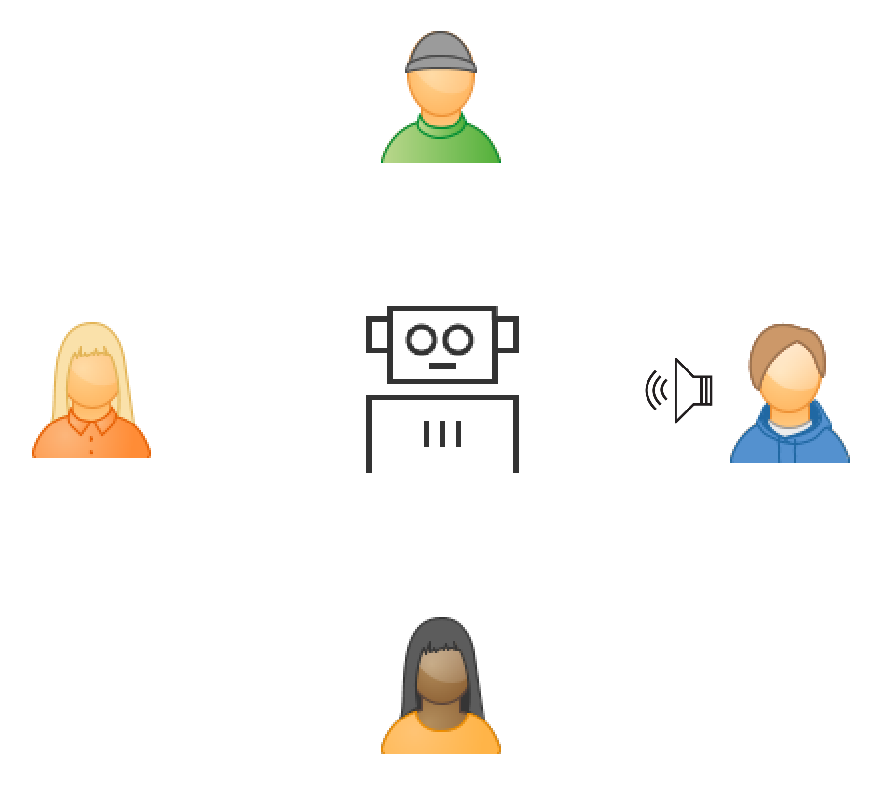
\includegraphics[width=0.5\textwidth]{diagrams/robocup_task_t1.pdf}
	}
	\caption{Test scenario for the RoboCup task}
	\label{pic:eval_task}
\end{figure}

\begin{figure}[]
	\centering
	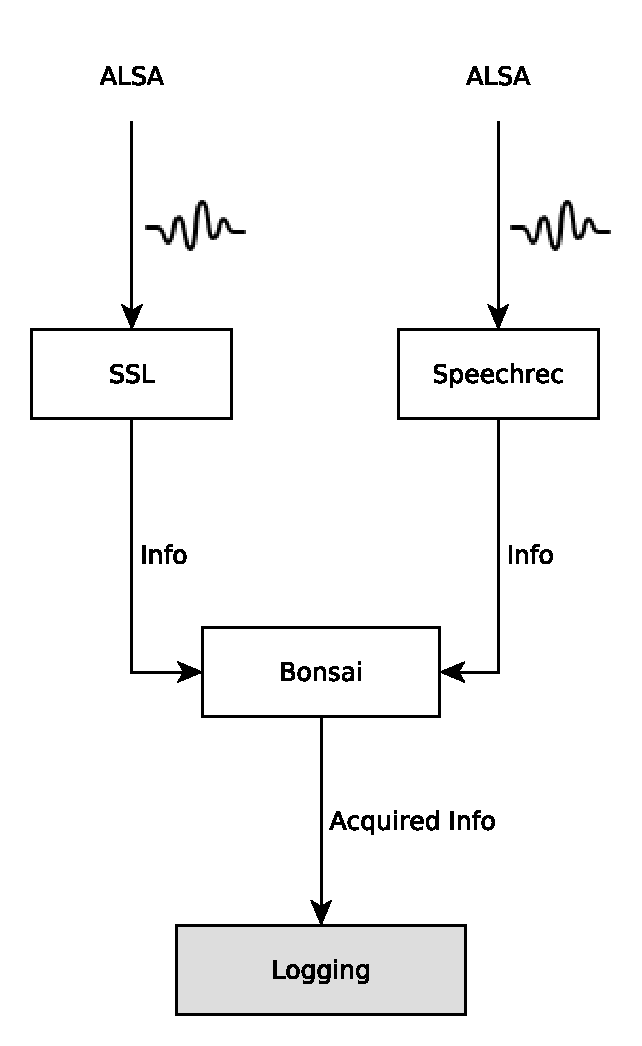
\includegraphics[width=0.5\textwidth]{diagrams/eval_task_old.pdf}
	\caption{Setup of existing solution}
	\label{pic:eval_task_setup_old}
\end{figure}

\begin{figure}[]
	\centering
	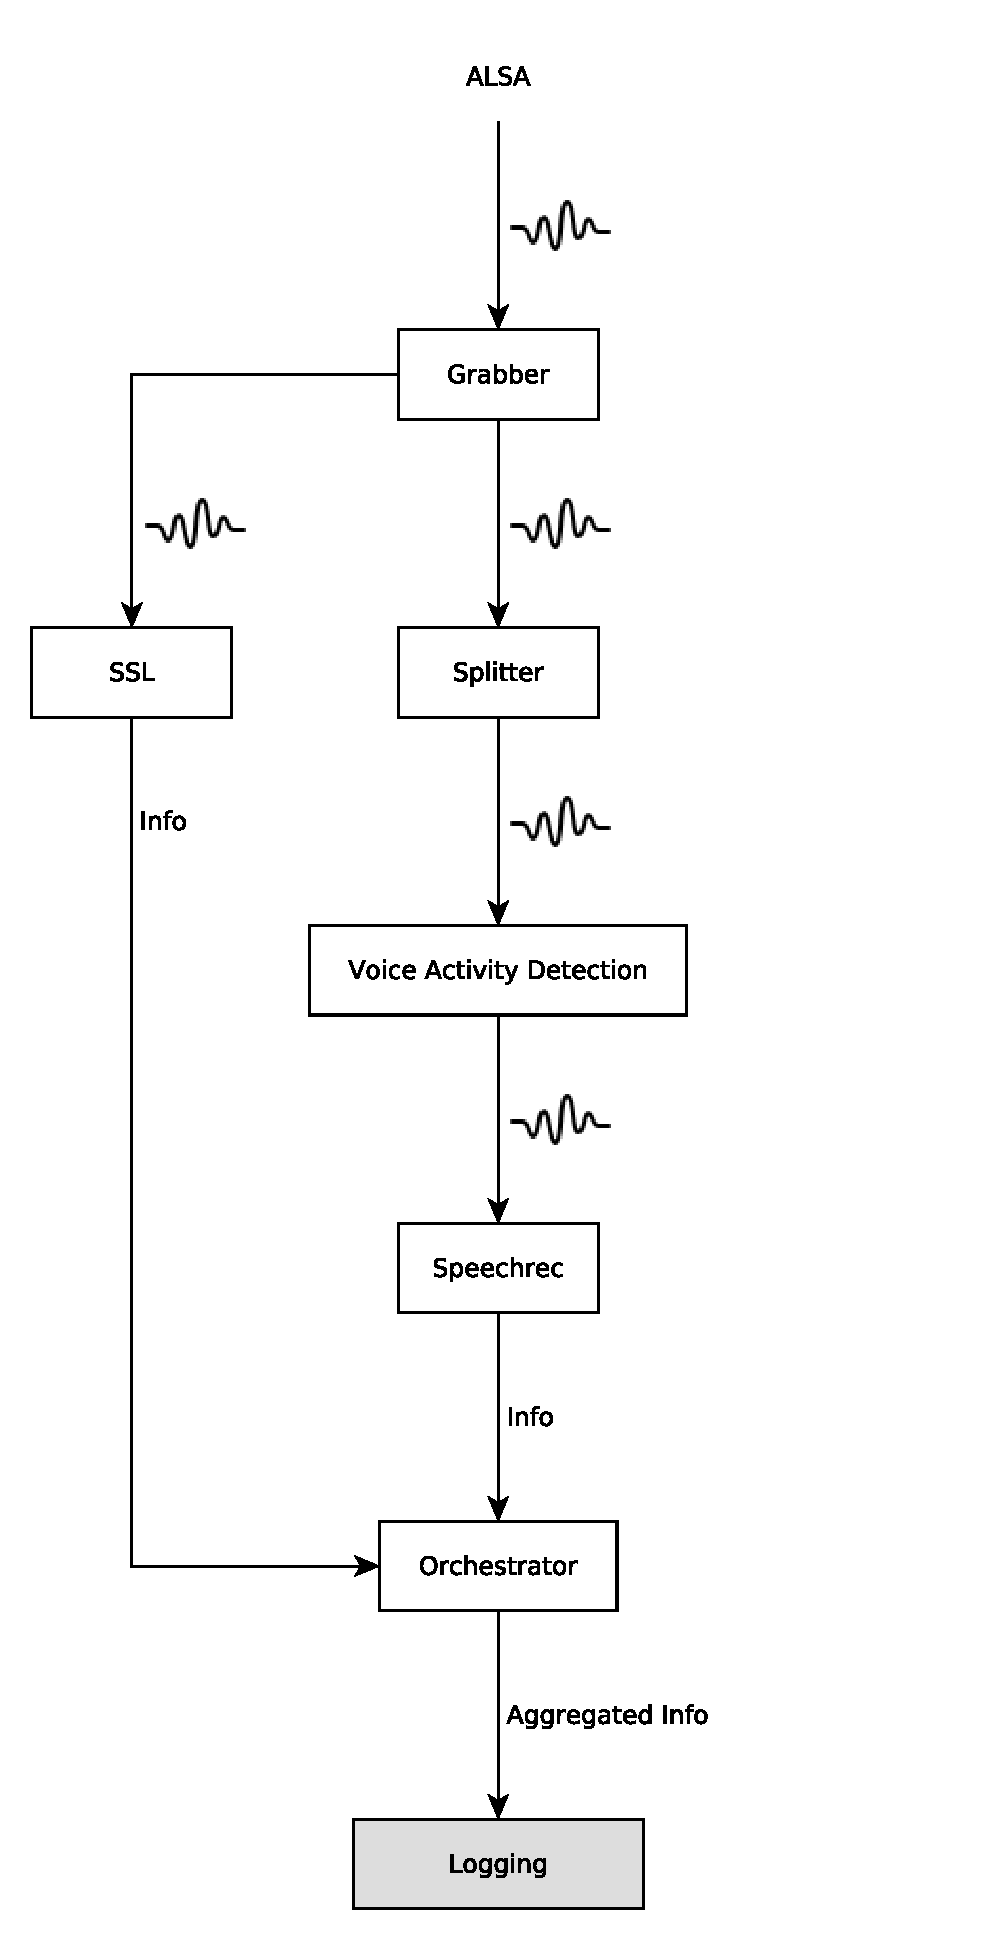
\includegraphics[width=0.5\textwidth]{diagrams/eval_task_proposed.pdf}
	\caption{Setup of of proposed pipeline}
	\label{pic:eval_task_setup_new}
\end{figure}

\begin{figure}[]
	\begin{tabular}{ | l | l | l | l |}
		\hline
		Run & Correctly recognized sentences & Points & Points by SSL \\ \hline
		1 & 50\% & 45 & 0 \\ \hline
		2 & 50\% & 40 & 10 \\ \hline
		4 & 35\% & 25 &  0 \\ \hline
		5 & 40\% & 30 & 10 \\ \hline
		6 & 45\% & 40 & 10 \\ \hline
		7 & 60\% & 50 & 10 \\ \hhline{|=|=|=|=|} 
		Avg & 46.7\% & 38.3 & 6.7 \\
		\hline
	\end{tabular}
	\caption{Results of the existing pipeline in the RoboCup task}
	\label{pic:eval_task_results_old}
\end{figure}

\begin{figure}[ht]
	\begin{tabular}{ | l | l | l | l |}
		\hline
		Run & Correctly recognized sentences & Points & Points by SSL \\ \hline
		1 & 65\% & 50 &  0 \\ \hline
		2 & 55\% & 70 & 20 \\ \hline
		4 & 55\% & 35 &  0 \\ \hline
		5 & 55\% & 50 & 20 \\ \hline
		6 & 60\% & 60 &  0 \\ \hline
		7 & 60\% & 60 & 10 \\ \hhline{|=|=|=|=|} 
		Avg & 58.3\% & 54.2 & 8.3\\
		\hline
	\end{tabular}
	\caption{Results of the proposed pipeline in the RoboCup task}
	\label{pic:eval_task_results_new}
\end{figure}
%!TEX root = thesis.tex
%=============================================================================


\chapter{Conclusion \& Future Work}
\label{conclusion}

I began this thesis with the goal to ultimately improve \gls{hri}, by providing robot behaviors with synchronized results and thus enable them to focus on perceiving humans better.
For this I created a framework which synchronizes and combines results of components of various disciplines, such as emotion and gender recognition.
Smaller, secondary goals were also formulated:
The solution was supposed to be modular, to increase its value for research.
Naturally, the solution should also perform as good as pre-existing solutions with regards to computational speed and accuracy.
This reiterated, I consider this thesis to be a mild success.

The RoboCup@Home experiment I could show my fusion approach to not only work, but to improve the accuracy of the used \gls{ssl} component in comparison to previously employed methods.
In this particular area, this thesis can be considered fully successful.
The data set experiment however is more of a mixed bag.
It inherently showed the proposed framework to be quite modular by its ability to incorporate additional components and reuse nearly all components from the RoboCup experiment.
On the other hand, it showed the proposed framework to be considerably slower then a comparable pre-existing solution.
I briefly investigated this problem and could determine the long computation time to be not be explainable by just the components and framework alone.
As such, I suspect an undiscovered bug to be he cause of this discrepancy.
Future work may thus begin by exploring this inconsistency and -if possible- eliminate it.

%--------------------

Apart from this, the logical next step would be to use the proposed framework to fed information into a robot behavior.
This way the work I presented can be properly utilized and thus improve \gls{hri} of robot, the very motivation for this thesis.
Another path for future work could start with creating more components for the proposed framework.
A number of the components I developed (see chapter \ref{main:components:start}) can not considered to be state of the art, but rather rapidly developed proofs of concept.
For productive work and actual research in the fields of speech recognition and robotics, especially multi-modal sensor fusion, as outlined in chapter \ref{related:fusion} it may prove fruitful to incorporate better performing algorithms into the proposed framework.

Another, rather unintentional feature of the proposed framework became clear when conducting the data set experiment.
The proposed framework provides a very easy way to benchmark different components against each other by providing distinct interfaces and as such a controls the environment of components to be benchmarked very tightly.
This way algorithms to be benchmarked can be controllably fed audio and their impact upon other components inspected.
It would for example be easily conceivable to test the word error rate of different combinations of \gls{vad} and \gls{asr} components.


\backmatter
%\printglossaries
\printbibliography[heading=bibintoc]

\appendix
%!TEX root = thesis.tex

%=============================================================================


\chapter*{Statement of authorship}

I hereby certify that this thesis has been composed by me and is based on my own work unless stated otherwise. 
No other person’s work has been used without due acknowledgment in this thesis. 
All references and verbatim extracts have been quoted, and all sources of information, including graphs and data sets, have been specifically acknowledged. 
This thesis has not been presented to an examination office in the same or a similar form yet.
\\\\\\\\
Bielefeld, \today
\\\\\\\\
Robert Feldhans

%=============================================================================
%\input{app_a}

\end{document}